\section{Systèmes d'administrations}\label{sec:rw:supervision:administration}
Depuis le début des années 80, grâce aux premières mises en réseau d'équipements, les systèmes d'administrations permettent de gérer des parcs de ressources. Le principe est de surveiller et surtout contrôler un système afin qu'il satisfasse les demandes des utilisateurs et les contraintes du propriétaire~\cite{Sloman:management}. Toutefois, afin d'administrer un système, la gestion des données qui décrivent le système est primordiale.

Cette section présente les systèmes d'administrations, qui sont encore déployés aujourd'hui pour exploiter des parcs de dispositifs à grande échelle. Ces systèmes sont spécifiés au travers de divers consortiums ou forums. Les principaux acteurs sont : le \textit{BroadBand Forum} (BBF) (portés par les opérateurs télécoms), le \textit{Forum Universal Plug'n'Play} (UPnP) (portés par l'électronique grand publique), ou encore \textit{Distributed Management Task Force} (DMTF), l'\textit{Institute of Electrical and Electronics Engineers} (IEEE) et l'\textit{Internet Engineering Task Force} (IETF), organisations ouvertes où participent entreprises, laboratoires et indépendants. Ces ententes permettent la spécification des standards autant au niveau des protocoles de communications que sur les modèles de données manipulés.

Cette section présente d'abord la structure et la gestion des données issues des ressources administrées. Ensuite, nous analysons l'ensemble des possibilités de traitement fournies par ce type de systèmes. Et enfin, une synthèse est présentée grâce à notre grille d'analyse.
\subsection{Gestion des données pour l'administration}
L'architecture de la gestion des données dans les systèmes classiques d'administration est principalement fondée sur des gestionnaires \enquote{agents}~\cite{CCITT:X700} (voir fig.~\ref{fig:rw:supervision:administration}). Cette architecture est celle utilisée de nos jours dans les protocoles d'administrations tels que TR-069~\cite{BBF:tr069}, UPnP Device Management~\cite{UPnP:DM2}, mais aussi sur des protocoles plus anciens tels que SNMP~\cite{IETF:SNMP}. Le principe est qu'un module logiciel est présent sur les dispositifs devant être administrés. Celui-ci comporte un agent capable de maintenir une petite \enquote{base de données} sous un format particulier représentant les données et états du système. Un gestionnaire est capable par la suite de transmettre les informations de l'agent à un système d'administration global. Ce dernier agrège ainsi l'ensemble des dispositifs.
\begin{figure}[ht]
    \centering
    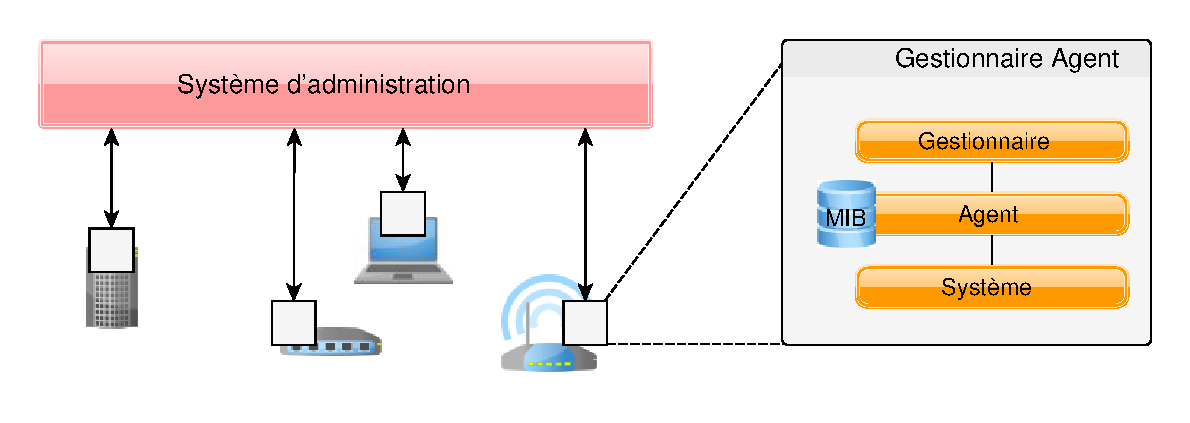
\includegraphics[width=.75\textwidth]{fig/rw-supervision-administration}
    \caption{Architecture d'un système classique d'administration}\label{fig:rw:supervision:administration}
\end{figure}

\subsubsection{Les données fournies par les agents}
Il existe plusieurs modèle de données dans le cadre des systèmes d'administrations. Le modèle le plus répandu reste la \textbf{structure hiérarchique}. La première apparition d'un tel modèle dans ce domaine remonte à la spécification de SNMP~\cite{IETF:SNMP} qui décrit le concept de \textit{Management Information Base} (MIB)~\cite{IETF:MIB}. Une \textit{MIB} est une base d'information où les données sont regroupées sous forme d'arbre. Chaque information possède un chemin unique (l'\textit{object identifier}) décrit par une suite de chiffres séparés de points.

Par exemple, \verb|1.3.6.1.2.1.2.2.1.2| est le chemin décrivant le nom d'une interface réseau sur un dispositif (par exemple \textit{eth0} sur un système Linux). Et le sous-arbre \verb|1.3.6.1.2| (MIB-II~\cite{IETF:MIB-II}) contient toutes les informations concernant les informations réseau du dispositif. Des catalogues répertorient désormais l'ensemble des \textit{MIB} existantes (standardisées ou non).

Les protocoles récents permettent aussi de manipuler des données de manière hiérarchiques sur les agents. Par exemple, dans le protocole TR-069, le modèle de données est décrit dans le rapport technique nommé \textit{TR-106}~\cite{BBF:tr106}. Dans le protocole UPnP-DM, le service de gestion de configuration (CMS)~\cite{UPnP:DMCMS} permet l'accès aux données. Dans ces derniers, le modèle de donnée est décrit comme un système de fichier. Les \textit{instances} sont assimilables à des dossiers, et les \textit{feuilles} sont assimilables à des fichiers. Les nœuds ont ainsi un nom et un chemin unique vers la racine \enquote{/}. 
\begin{figure}[ht]
    \centering
    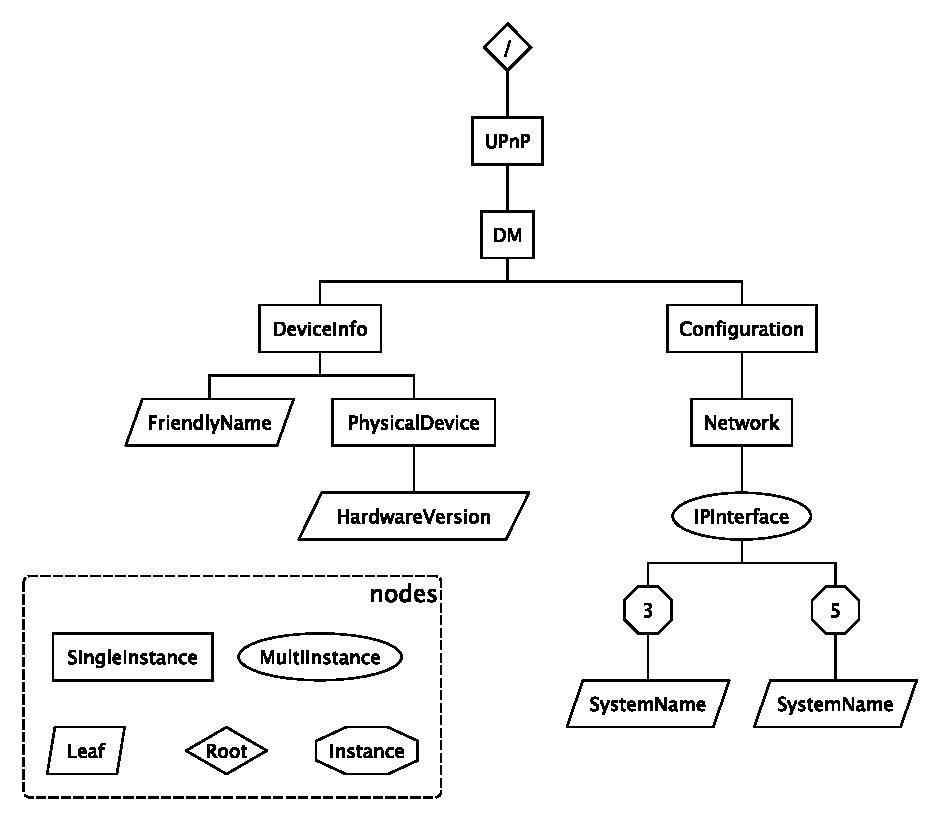
\includegraphics[width=.6\textwidth]{fig/rw-supervision-dmtree}
    \caption{Structure hiérarchique du modèle de données d'UPnP-DM}\label{fig:rw:supervision:dmtree}
\end{figure}

Un exemple de modèle de données de ce type de structure est présenté en figure~\ref{fig:rw:supervision:dmtree}. Une donnée est donc définie de manière unique, tout comme dans une \textit{MIB}, grâce à son chemin complet. Dans le vocabulaire du domaine de l'administration, cette donnée est appelée \textit{paramètre}. Le \textit{chemin} d'un paramètre est la concaténation des noms des nœuds qui le sépare de la racine, avec pour séparateur \enquote{/} dans UPnP ou \enquote{.} dans TR-069. L'implémentation de l'agent permet de créer et de remplir cette base d'information.

\begin{figure}[ht]
    \centering
    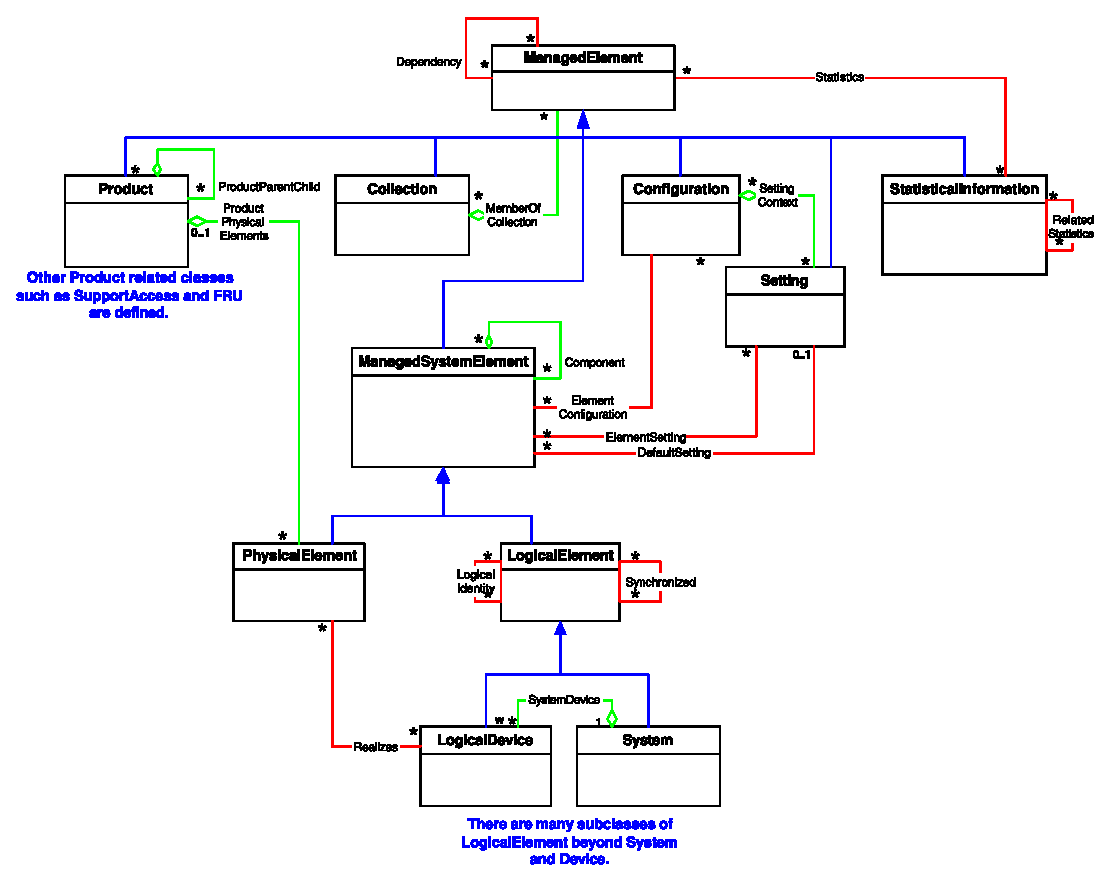
\includegraphics[width=.6\textwidth]{rw-supervision-cimcore}
    \caption{Modèle de classe de la partie \textit{Core} de \textit{CIM}}\label{fig:rw:supervision:cimcore}
\end{figure}
Toutefois, tous les modèles ne sont pas structurés sous forme de hiérarchie. Par exemple, la DMTF a adopté l'approche objet. En effet, dans les protocoles tels que WBEM~\cite{DMTF:WBEM} ou WS-MAN~\cite{DMTF:WS-MAN}, le modèle \textit{CIM} (\textit{Common Information Model})~\cite{DMTF:CIM} est décrit par un diagramme de classe UML comme présenté en figure~\ref{fig:rw:supervision:cimcore}. Ces protocoles sont notamment utilisés pour l'administration de web-services et applications entreprises. 

Plusieurs extensions standardisées existent pour modéliser les différents aspects des systèmes observés : Base de données, Dispositifs, Réseau, Sécurité, Utilisateur, Applications\dots{} Ainsi, le modèle de données est un modèle d'objet respectant l'ensemble des spécifications et des extensions. L'inconvénient majeur d'un tel choix reste la complexité de \textit{CIM} qui se trouve souvent réduite pour être applicable en pratique~\cite{Lopez:datacenter}.

Le système se compose ainsi de multiples agents qui sont une représentation de chaque objet. Les objets du système sont ainsi exposés à un service de gestion pour fournir plusieurs propriétés. Nous pouvons noter que ce principe reste le même pour l'administration de modules Java dans le protocole JMX~\cite{Sun:JMX} où des objets particuliers (les \textit{MBean}) sont exposés et peuvent être consultés et manipulés via ce protocole.

\subsubsection{Gestion de l'évolution des données}
Pour les différentes solutions présentées, les agents ont toujours trois modes principaux pour fournir des données :
\begin{itemize}
	\item[\textbf{Consultation indirecte}: ] Ce fonctionnement est le plus simple. La donnée est stockée dans une base d'information. Au moment de la consultation, l'agent lit directement dans la base et renvoie l'information.
	\item[\textbf{Consultation active}: ] Au moment de la consultation de la données via un primitive comme \enquote{\it get}, l'agent va effectuer le relevé actif de la donnée à la source. Ce relevé peut potentiellement prendre plus de temps qu'une simple lecture dans une base d'information.
	\item[\textbf{Événement}: ] La plupart des systèmes d'administrations supportent un mécanisme de \textit{publish}/\textit{subscribe} permettant de créer des canaux d'événements. La création d'événement se fait à partir du changement de valeur d'un paramètre ou à la création d'objets (ou de chemins).
\end{itemize}

Le problème majeur est que la consultation et les canaux d'événements sont deux approches et deux mécanismes différents qui sont rarement intégrés.

\subsubsection{Le gestionnaire global}
Dans l'architecture présentée en figure~\ref{fig:rw:supervision:administration}, de multiples agents fournissent différentes informations selon les modèles présentés dans la section précédente. Le système d'administration se connecte aux différents agents afin de les administrer. Il sert à la fois d'interface à l'utilisateur et d'infrastructure de collecte et d'analyse. Ainsi, il constitue la vue globale du système par l'intégration des données.

Il est important de noter que ce système peut ne pas être centralisé pour mieux amortir la charge en la présence de grandes quantités d'agents à administrer. Toutefois, pour l'administration de dispositifs des architectures centralisées peuvent suffire. Par exemple, pour l'administration de ses dispositifs, \textit{France Telecom} utilise un \textit{ACS} (\textit{Auto-configuration Server}, serveur d'administration en TR-069) centralisé. En effet, la fréquence d'émission des données en fonctionnement normal est lente (pour chaque dispositif, un rapport par jour typiquement). Pour les 10 millions d'équipements à gérer, une capacité de 500 réceptions par seconde côté serveur est suffisante. Cette capacité est atteinte sur des \textit{ACS} récents tels que \textit{EDGE}~\cite{Motorola:EDGE} de \textit{Motorola} sur des serveurs de puissance moyenne.

Toutefois, plus l'usage le requiert, plus ce type d'architecture ne peut supporter la charge des informations remontées. Plusieurs systèmes d'administrations proposent des architectures décentralisées (principalement hiérarchiques) pour la gestion à plus grande échelle~\cite{Kessis:management}. La hiérarchie peut se découper par lieu géographique, ou par domaine d'activité.

Nous venons de voir comment les systèmes d'administrations sont structurés et notamment comment ces systèmes modélisent leurs données. La section suivante présente les capacités de traitements de ce type de systèmes.

\subsection{Possibles traitements de données}
Que ce soit au niveau de l'agent comme au niveau du gestionnaire global, les données peuvent être traitées. Cette section détaille les différentes possibilités. Tout d'abord, nous voyons comment l'hétérogénéité des systèmes est traitée et comment l'intégration des multiples agents se fait. Par la suite, nous détaillons l'ajout de nœuds particuliers comme calcul de statistiques ou l'ajout de fonctions tierces.

\subsubsection{L'hétérogénéité par l'uniformisation des modèles}
La standardisation est un enjeux majeur pour les systèmes d'administrations à grande échelle. Comme présentés précédemment, la spécification les protocoles d'administrations des agents se fait autour de consortiums. Ainsi, l'hétérogénéité des systèmes est gérée par le fait qu'il est supposé acquis que les standards soient respectés. Suivant les dispositifs observés, différents profils existent. Que ce soit pour les profils hiérarchiques ou à objet, des spécifications sont écrites pour décrire le modèle de données.

Le nombre de spécification augmente énormément pour essayer de limiter l'hétérogénéité. Par exemple, dans le cadre de \textit{TR-069}\footnote{Pour rappel, ce protocole est établit par un consortium d'opérateurs télécoms : le BBF}, il existe seulement 9 profils principaux. Mais lorsque les domaines d'activités s'élargissent le nombre d'entités devient difficile à contrôler, comme dans CIM où le nombre de spécifications est de 16\footnote{Sachant que les spécifications CIM sont bien plus complexes et possèdent plus d'entités.}, ou dans les MIB qui sont au nombre de 318 spécifiées par l'IETF.

Donc, la gestion de l'hétérogénéité se fait par la description de profils standardisés. Toutefois, la standardisation entraine des problèmes de complexité. Ce qui rend sa maîtrise plus difficile pour les utilisateurs.

\subsubsection{Intégration de sources}
L'avantage principal d'utiliser des modèles standards est l'intégration des sources de données. En effet, comme chacune des entités du système répond à un profil prédéfini, il est possible de faire l'union des données par catégorie pour avoir toutes les entités répondants aux différents profils. Ainsi, les données sont naturellement intégrées dans un modèle commun, ce qui permet aux concepteurs de systèmes d'observations de fournir des fonctions très avancées sans pour autant connaître l'instance du système. De plus, plusieurs protocoles et standards peuvent être utilisés dans un même système, comme l'a proposé WBEM, dans lequel des objets SNMP, JMX et autres sont intégrés à un modèle commun CIM.

Une fois les données accessibles à un niveau global, il devient possible de traiter ces données afin de les analyser, ou former des alertes. Pour cela, les systèmes d'administrations ne fournissent pas tous les mêmes capacités. Par défaut, la seule capacité que peut fournir l'agent est la récupération de son modèle de données (ou une sous-partie). Cependant, plusieurs systèmes permettent à l'utilisateur de définir des processus plus complexes pour permettre un traitement de plus haut niveau.

L'approche la plus utilisée est le \textit{scripting}. Le système d'observation fournit à l'utilisateur un langage \textbf{impératif} qui lui permet de définir des routines. Par exemple, EDGE~\cite{Motorola:EDGE} fournit une interface \textit{Javascript}, et l'\textit{ACS} d'\textit{Alcatel-Lucent} permet d'utiliser des programmes \textit{Python}. Ces routines peuvent par la suite être intégrées dans des réponses aux événements, ou dans des procédures de diagnostics ou encore de configuration.

Il est notable que les standards WBEM et WS-MAN définissent un langage \textbf{déclaratif} de manipulation de modèles CIM, le \textit{CQL} (\textit{CIM Query Language})~\cite{DMTF:CIM-QL}. Ce langage est très similaire à \textit{SQL} utilisé dans un cadre relationnel-objet. Dans sa spécification, il permet toutes les fonctionnalités de \textit{SQL} (sélection, projection, jointure, agrégation, imbrication de requêtes). Il est aussi utilisé afin de définir des filtres plus précis sur les événements (en remplacement du langage par défaut \textit{XPath}). Il est intéressant de noter que ce langage permet aussi la définition de \textit{politiques de gestions}, assimilables à des routines événements-condition-action. Toutefois, il reste peu implémenté dans la pratique.

\subsubsection{Sur l'agent : statistiques et extension}
Dans chacune des solutions présentées, il existe des parties du modèle des données consacrées à la présentation de statistiques. En effet, pour un paramètre dont la valeur représente une mesure, il peut être intéressant de fournir des extremums ou moyennes calculées à la volée. Plusieurs standardisations existent pour permettre un tel calcul principalement sur un échantillon précis ($N$ données) avec un ensemble fixé d'opérateurs.

Tous les modèles présentés sont extensibles à volonté par les constructeurs des dispositifs. Par exemple, sous UPnP-DM et TR-069, il est autorisé de rajouter des branches à l'arbre de données sous l'appellation \verb|X_{ORGANISATION}| (par exemple \verb|X_ORANGE_COM|). Ainsi, cela permet aux constructeurs de fournir des données non prévues dans les standards ou pour rajouter des fonctionnalités de traitement.

\subsection{Synthèse}

\begin{table}[!ht]
\criteretabDonnee
    {Principalement structure \textbf{hiérarchique} sous forme de système de fichier. Quelques systèmes d'administration utilisent des modèles objets avec \textit{CIM}, mais restent difficile à maîtriser.}
    {Les différentes entités du systèmes sont des nœuds du modèle. Pas de contraintes ou d'inférences exprimables.}
    {Le dynamisme est géré par le mode d'accès. Certaines données peuvent être notifiables. Les mécanismes d'interrogations sont séparés.}
\criteretabTraitement
    {Instantanée et continue sur certaines données. Pas d'hybride possible vu que les procédés sont très séparés.}
    {Standardisation des modèles. Toutes les entités sont structurés dans le même formalisme. Intégration par union des données pour chaque profil.}
    {Appel de méthodes standardes pour récupérer un sous-arbre du modèle. Code impératif (scripting) principalement pour manipuler les données au niveau du gestionnaire. Utilisation de langage déclaratif (similaire SQL ou XPath) possible.}
    {Procédures à écrire en \textit{script}. Projection, sélection et union principalement. Certains nœuds particuliers permettent de calculer des statistiques.}
\criteretabAdaptabilite
    {Pas d'adaptation spécifique car les dispositifs doivent implémenter des standards.}
    {Pas de perspectives métiers en dehors de la sélection sur les branches du modèle.}
    {Nœuds particuliers pour le calcul. Fonctions métiers intégrées dans le gestionnaire.}
    {Très efficace et utilisé pour gérer des parcs de millions de dispositifs.}
\caption{Synthèse des systèmes d'administration}\label{tab:rw:supervision:administration:synthese}
\end{table}

Le tableau~\ref{tab:rw:supervision:administration:synthese} résume l'ensemble de l'analyse pour les systèmes d'administrations. L'ensemble permet effectivement beaucoup de fonctionnalité pour les utilisateurs. Le choix d'approches principales à base de standard fait que ces systèmes sont actuellement très répandus pour gérer des systèmes de tous types. Ce qui en fait un excellent système pour collecter les données sur les ressources du système. Toutefois, le traitement des données est principalement faite dans un langage non-déclaratif. De plus, les canaux événementiels et la consultation des bases d'informations sont gérés dans des approches et mécanismes très différents. Ceci rend une observation intégrée difficile.